% !TEX root = main.tex
\section{Aufbau und Durchführung des Versuchs}
\label{sec:Aufbau}
Für die Messungen der Frequenz- bzw. Geschwindigkeitsspektren astronomischer Objekte in der Milchstraßenebene wurde das Radioteleskop ,,Brage``, welches in Abbildung \ref{fig:Tesleskop} dargestellt ist, des \textsc{Onsala Space Observatory} in Schweden genutzt.
Dazu wurden das Teleskop der \textsc{Salsa}-Onsala-Einrichtung per Remote-Steuerung bedient und dabei interne Software der Forschungsanstalt genutzt.\\
\begin{figure}[H]
    \centering
    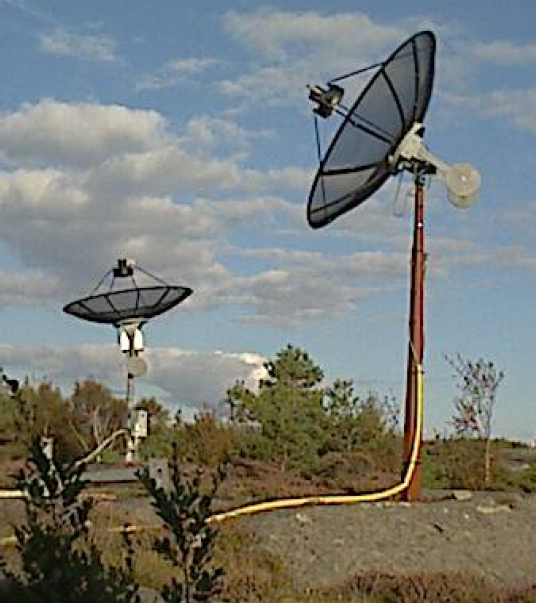
\includegraphics[width=0.5\textwidth]{pngplots/Teleskop.png}
    \caption[Radioteleskope]{Fotografie der beiden Radioteleskope ,,Brage`` und ,,Vale`` in Onsala, Schweden. Entnommen aus \cite{Usermanual}.}
    \label{fig:Tesleskop}
\end{figure}

Gemäß der Dokumentationen \cite{Usermanual} und \cite{AntennaResp} beträgt der Durchmesser des Teleskops $\SI{2.3}{\metre}$. Die Track-Genauigkeit wird auf $\SI{0.5}{\degree}$ und das Auflösungsvermögen auf $\SI{6}{\degree}$ bei $\SI{1420}{\mega \hertz}$ beziffert.
Zur Erstellung von präzisen Spektren ist eine Bandbreite von $\SI{2}{\mega \hertz}$ mit 256 Kanälen verwendet worden, dabei beträgt die Frequenzauflösung pro Kanal $\SI{7.8}{\kilo \hertz}$.
Da \textsc{Salsa} noch nicht Flux-kalibriert ist, werden Intensitäten stets in ,,arbitrary units`` angegeben und bei der Messung von Antennen-Temperaturen sind nur Betrachtungen relativer Werte aussagekräftig.
Zudem sollten zum Erhalt guter Spektren stets Bereiche über $\SI{15}{\degree}$ horizontaler Höhe und Messdauern von über $\SI{20}{\second}$ -- bei den Sonnenmessungen genügen bereits $\SI{10}{\second}$ -- beachtet werden. Eine Betrachtung unterhalb dieser Höhe und Zeit würde ein zu großes Rauschen in den Spektren erzeugen. Zudem können aufgrund der geographischen Lage des Teleskops nicht alle Bereiche der Milchstraße vermessen werden, da von diesen keine Strahlung zum Teleskop gelangt.
%Welche Bereiche waren nicht betrachtbar?Das hab ich bei mir später schon drinnen. Brauchen wir hier glaube ich nicht extra.
Für die Vermessungen von Milchstraße und Sonne konnten verschiedene Frequenzen betrachtet werden ($\SI{1420.4}{\mega \hertz}$ respektive $\SI{1410}{\mega \hertz}$) sowie zwischen  ,,Switched`` - -- zur Minderung von Rauschen --  und ,,Signal`` -Modus -- zur besseren Intensitätsmessung -- gewechselt werden.
Zudem konnten je nach Anforderung galaktische Koordinaten übergeben oder spezielle astronomische Objekte wie die Sonne direkt getrackt werden.
Auch azimutaler und Höhenoffset sowie die Messdauer waren einstellbar.\\ 
\\ 
In Vorbereitung der Messungen wurde mittels des Programms \textsc{Stellarium} der am Messtag, 13. Mai, zur Messzeit zwischen 7 und 13 Uhr vermessbare Bereich der Milchstraße ermittelt.
Am Versuchstag wurden dann zunächst die Areale der Milchstraße vermessen, welche als Erste den beobachtbaren Bereich verlassen.
Hierfür wurde stets eine Messdauern von $\SI{60}{\second}$ veranschlagt.
Dabei wurden in Schritten von $\SI{5}{\degree}$ galaktischer Länge von $\SI{33}{\degree}$ bis $\SI{103}{\degree}$, jeweils bei $\SI{0}{\degree}$ galaktischer Breite und im ersten Quadranten ($\SI{0}{\degree} \le l \le \SI{90}{\degree}$ galaktischer Länge) auch bei $b=\pm \si{2}{\degree}$, Spektren aufgezeichnet.
Anschließend wurden die Belichtungsdauern bei fester galaktischer Länge ($\SI{84}{\degree}$) und Breite ($\SI{0}{\degree}$) zwischen $\SI{1}{\second}$, $\SI{3}{\second}$, $\SI{10}{\second}$, $\SI{30}{\second}$, $\SI{100}{\second}$ und $\SI{300}{\second}$ variiert.
Dann wurden in Schritten von $\SI{10}{\degree}$ galaktischer Länge von $\SI{113}{\degree}$ bis $\SI{203}{\degree}$ jeweils bei $\SI{0}{\degree}$ galaktischer Breite Spektren aufgezeichnet.
Zuletzt wurden, bei möglichst hohem Sonnenstand, folglich möglichst zu lokaler Mittagszeit Spektren der Sonne gewonnen.
Dabei wurde stets eine Messdauern von $\SI{10}{\second}$ beachtet.
Zum einen wurde ein Raster durch 25 Messungen generiert.
Dabei wurden eine relative Weite des Rasters von $\SI{5}{\degree}$ genutzt und durch azimutalen und Höhenoffset relativ zur Sonne das Raster erstellt.
Zum anderen wurde ein Kreuzscan der Sonne durchgeführt.
Dabei wurde in $\SI{2}{\degree}$-Schritten von $\SI{-16}{\degree}$ bis $\SI{16}{\degree}$ relativem Offset sowohl in Azimut wie in Altitude gemessen. Die jeweils andere Größe wurde auf $\SI{0}{\degree}$ Offset gesetzt.